% !TEX root = BA-Bauer.tex

\subsection{Gehäusedesign}
Mit dem Gehäuse wird aus der abstrakten Platine ein vorzeigbares Produkt. Wichtig ist nicht nur die Optik sondern auch das Design in funktioneller Sichtweise. Das beschriebene Platinendesign in Kapitel \ref{sec:PCB-Design} und 3D-Modell bildet die Basis für die Entwicklung des Gehäuses und kann durch die Verbindung von $EAGLE$ mit der 3D-CAD-Software $Fusion360$ direkt in die Konstruktion virtuell  eingefügt werden. Damit kann sichergestellt werden, dass z.B. Bohrungen im Gehäuse mit den in der Platine befindlichen übereinstimmen und das die Bauteile auf der Platine nicht mit dem Gehäuse Kollidieren. Die Konstruktion ist auf die Fertigung im 3D-Druckverfahren ausgerichtet, da damit in kurzer Zeit Iterationen des Designs kostengünstig gefertigt werden können. Bei dem verwendeten Material handelt es sich um den biologisch abbauaren Kunststoff $Poly-lactid-acid$ (PLA). Er ist einfach zu drucken, nachzubearbeiten, kostengünstig in der Anschaffung und besitzt eine ausreichende Stabilität.

Abbildung \ref{fig:Housing-front} und \ref{fig:Housing-back} zeigen das 3D-Modell des Gehäuses, dessen grundsätzliches Design simpel und kompakt ist (15,7\,cm breit, 8,14\,cm tief und 5,25cm hoch). Die Breite und Tiefe des Gehäuses werden nahezu komplett von der Platine ausgefüllt. Die Höhe des Gehäuses wird von den XLR-Buchsen vorgegeben und ist daher besonders im vorderen Teil nicht voll ausgenutzt. Bei einer Weiterentwicklung könnte dieser freie Platz für einen integrierten Akku genutzt werden. Der Boden des Gerätes verläuft parallel zur Platine damit die eingesteckten Kabel rechtwinklig zur Tischoberfläche verlaufen und sie somit das Gerät druch ihr Eigengewicht nicht zum kippen bringen. Auf der Oberseite befindet sich das LCD-Modul, die LEDs, Taster und der Encoder. Über den LEDs befinden sich weiße Diffusionsscheiben, die das Licht der darunterliegenden LEDs brechen und somit das Leuchten aus größerer Distanz und einem größeren Blickwinkel sichtbar machen. Auf der Rückseite befinden sich die XLR-Buchsen und eine vielzahl von Schlitzen, die einen Luftaustausch ermöglichen und einen Hitzestau vorbeugen. Auf der linken Seite befindet sich der SD-Kartensteckplatz und USB-Anschluss.
\begin{figure}[h]
	\begin{minipage}{.45\linewidth}
		\centering
		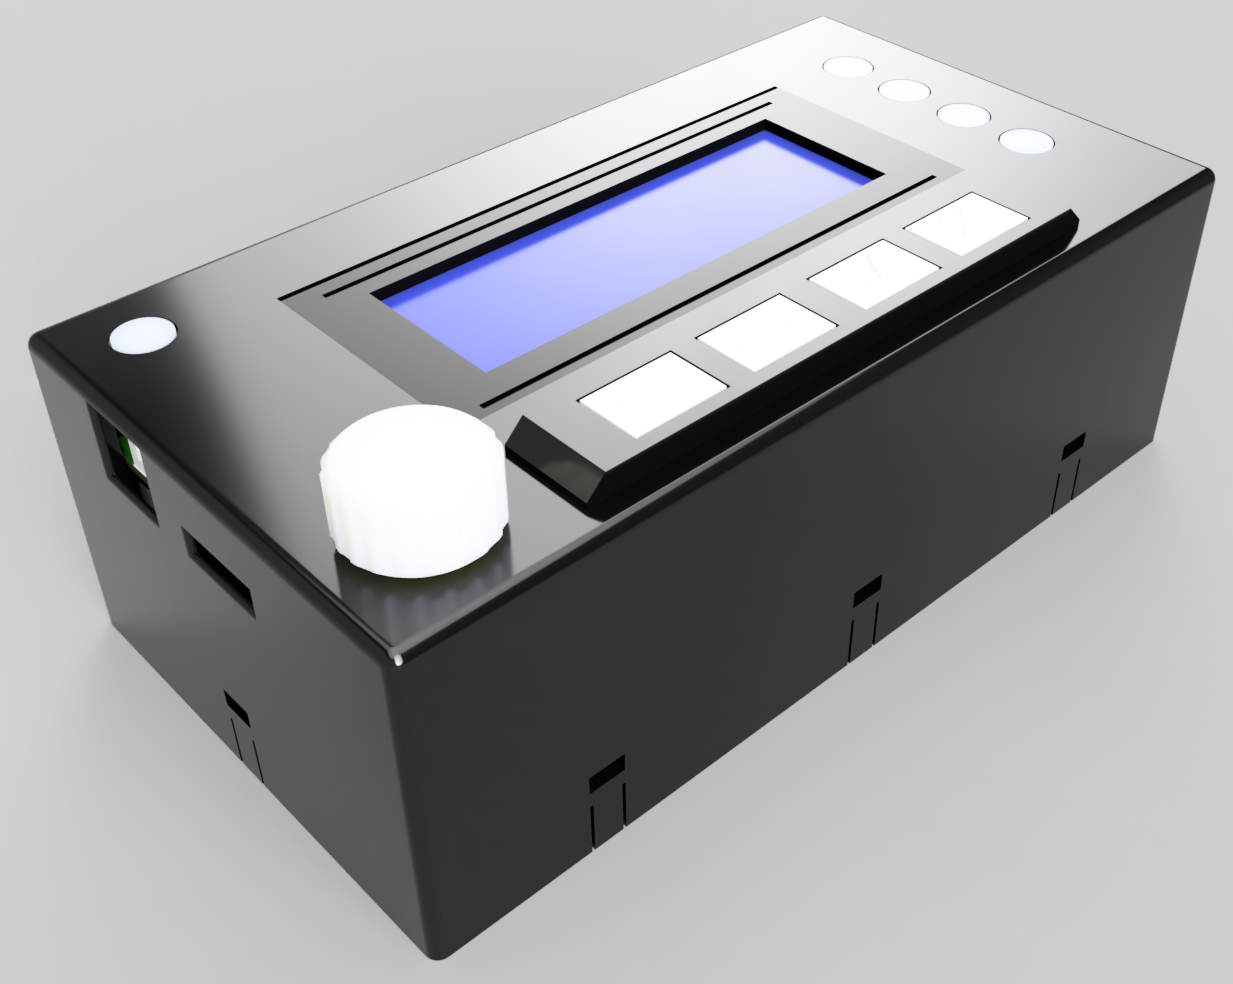
\includegraphics[height=.2\textheight]{Housing-front}
		\caption{Gehäuse 3D-Modell Frontseite}
		\label{fig:Housing-front}
	\end{minipage}
	\hfill
	\begin{minipage}{.45\linewidth}
		\centering
		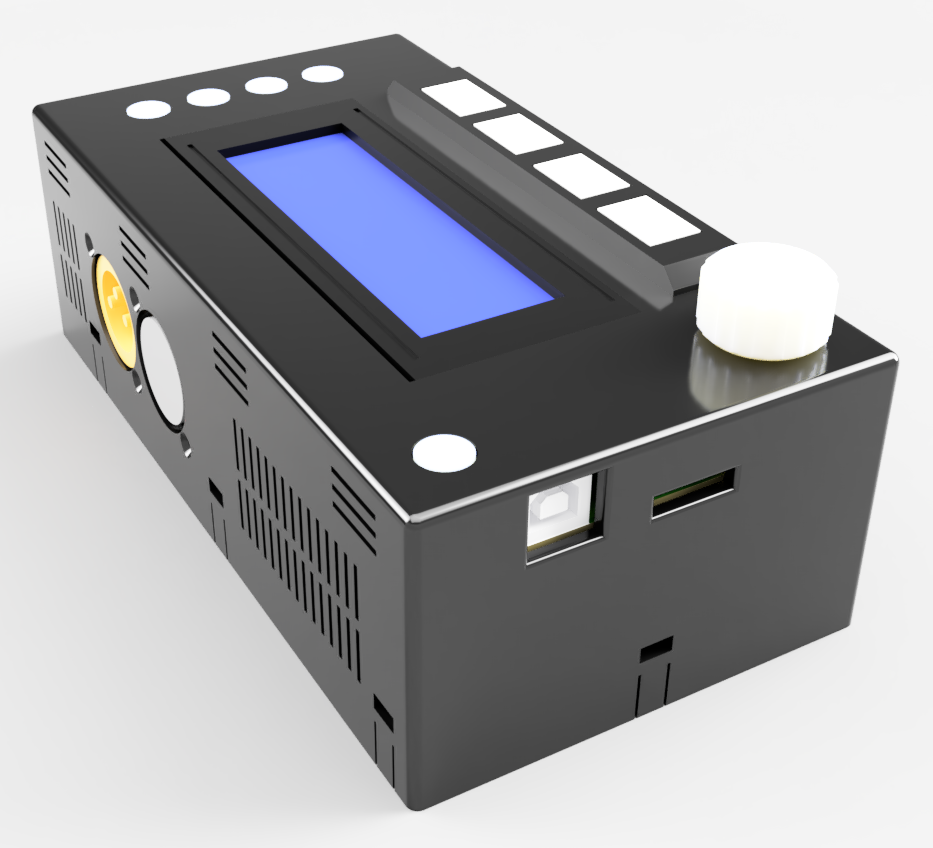
\includegraphics[height=.2\textheight]{Housing-back}
		\caption{Gehäuse 3D-Modell Rückseite}
		\label{fig:Housing-back}
	\end{minipage}
\end{figure}
Die Platine muss ausreichend im Gehäuse befestigt sein damit sie sich beim Betätigen der Taster nicht verbiegt und somit das Betätigen erschwert bzw. unmöglich macht. Abbildung \ref{fig:Housing-Befestigung} und \ref{fig:Housing-Befestigung2} zeigen Schnittanalysen des 3D-Modells. Für einen größtmöglichen Halt der Platine im Bereich der Taster wird die Platine in einen Schlitz im Gehäuse eingeführt (rot markiert). Durch den Schlitz wird die Auflagefläche erhöht und die durch einen Tastendruck einwirkende Kraft auf sie verteilt. Auf der gegenüberliegenden Seite wird die Plaitine mithilfe von Schrauben mit M3-Gewinde befestigt (blau markiert). Dazu befinden sich zylinderförmige Extrusionen an der Oberseite, die mittig eine Bohrung mit einem M3 Gewinde besitzen. Zudem befinden sich auf der gleichen Seite Ausschnitte für die XLR-Buchsen, welche außerdem mit dem Gehäuse verschraubt werden, zu sehen in Abbildung \ref{fig:Housing-back}. Mit der grün markierten Bohrung wird das LCD-Modul mit den bereits vorhanden Löchern verschraubt. Abstandshalter zwischen LCD-Modul und Platine ermöglichen die Verschraubung von der Unterseite der Platine.
\begin{figure}[h]
	\begin{minipage}{.35\linewidth}
		\centering
		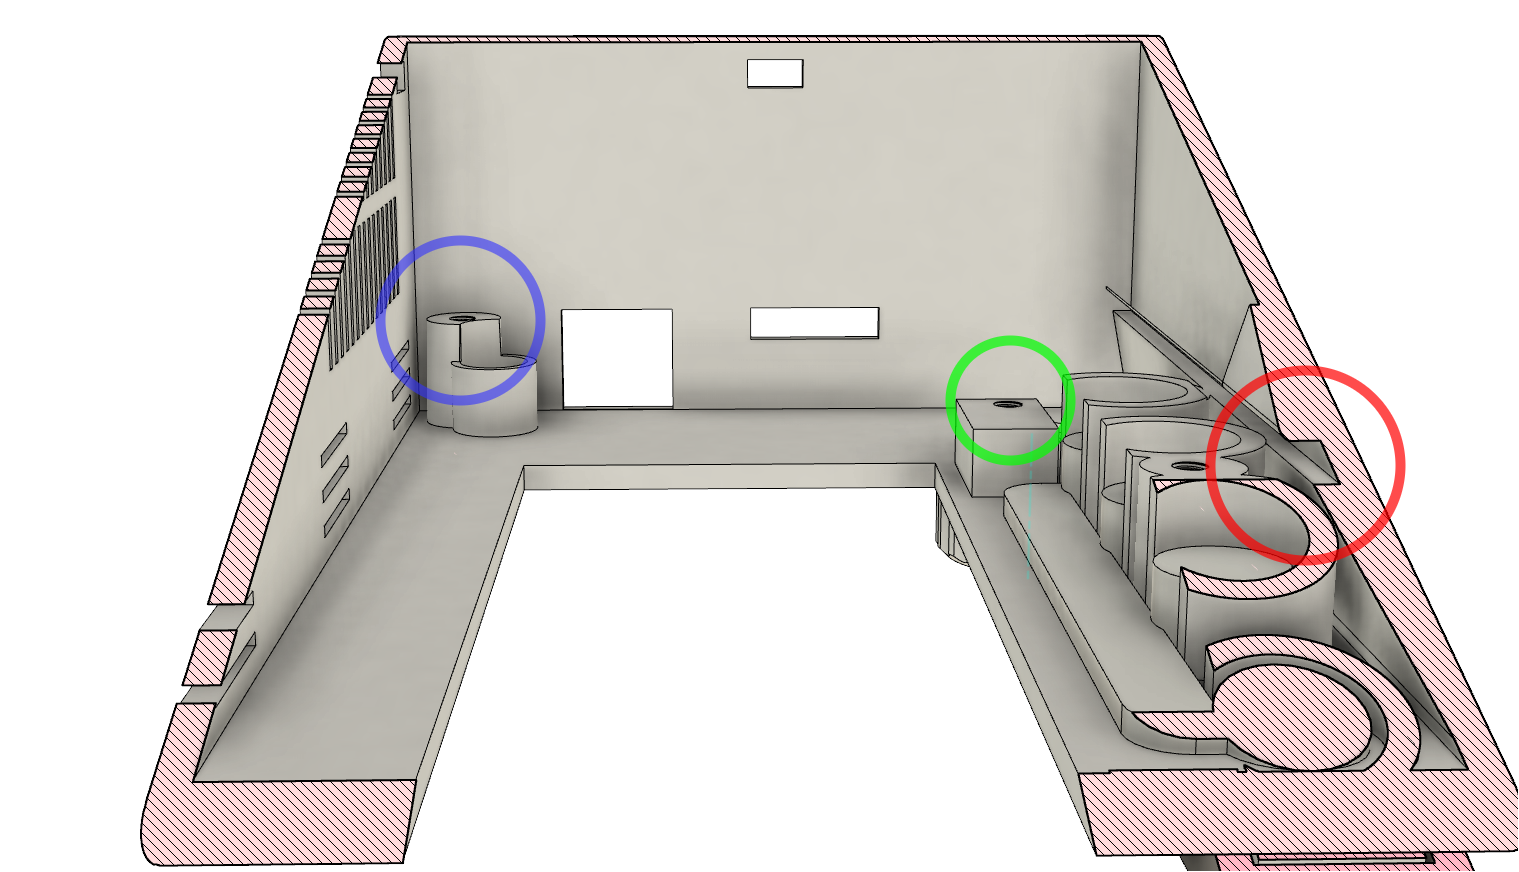
\includegraphics[height=.13\textheight, angle=180]{Housing-Schnitt-Befestigung-mark}
		\caption{Gehäuse Schnitt}
		\label{fig:Housing-Befestigung}
	\end{minipage}
	\hfill
	\begin{minipage}{.55\linewidth}
		\centering
		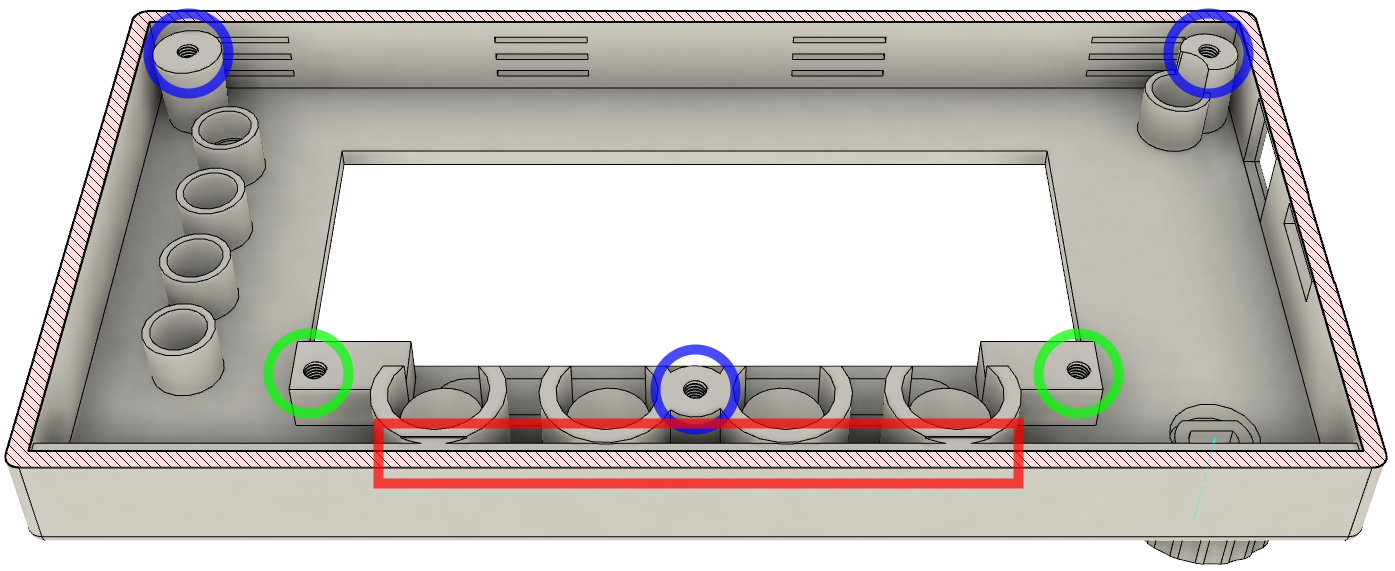
\includegraphics[height=.13\textheight, angle=180]{Housing-Schnitt-Befestigung2-mark}
		\caption{Gehäuse Schnitt Draufsicht}
		\label{fig:Housing-Befestigung2}
	\end{minipage}
\end{figure}
Damit die Platine im Gehäuse plaziert und befestigt werden kann, muss das Gehäuse geöffnet werden können. Um bei der Entwicklung möglichst unkompliziert die Platine erreichen zu können, befindet sich ein Clip-Mechanismus an der Unterseite des Gerätes, mit dem der Boden einfach entfernt werden kann. Abbildung \ref{fig:Housing-clip-side} zeigt die Seitenansicht des Mechanismusses. In der Oberseite des Gehäuses befinden sich Rechteckige Aussparungen in die die an der Unterseite befindlichen Clips einhaken können. Durch das verwendete 3D-Druckverfahren sind die Clips eine Schwachstelle der Konstruktion, da PLA verhältnismäßig spröde ist und die Clips beim einhaken in die Aussparungen leicht gebogen werden müssen. Um das Material beim verbiegen weniger zu belasten ist die Länge der Clips bis in den Boden hinein verlängert. Dadurch wird das Material auf eine längere Strecke hinweg gebogen und das Biegemoment somit verteilt.
\begin{figure}[h]
		\begin{minipage}{.45\linewidth}
		\centering
		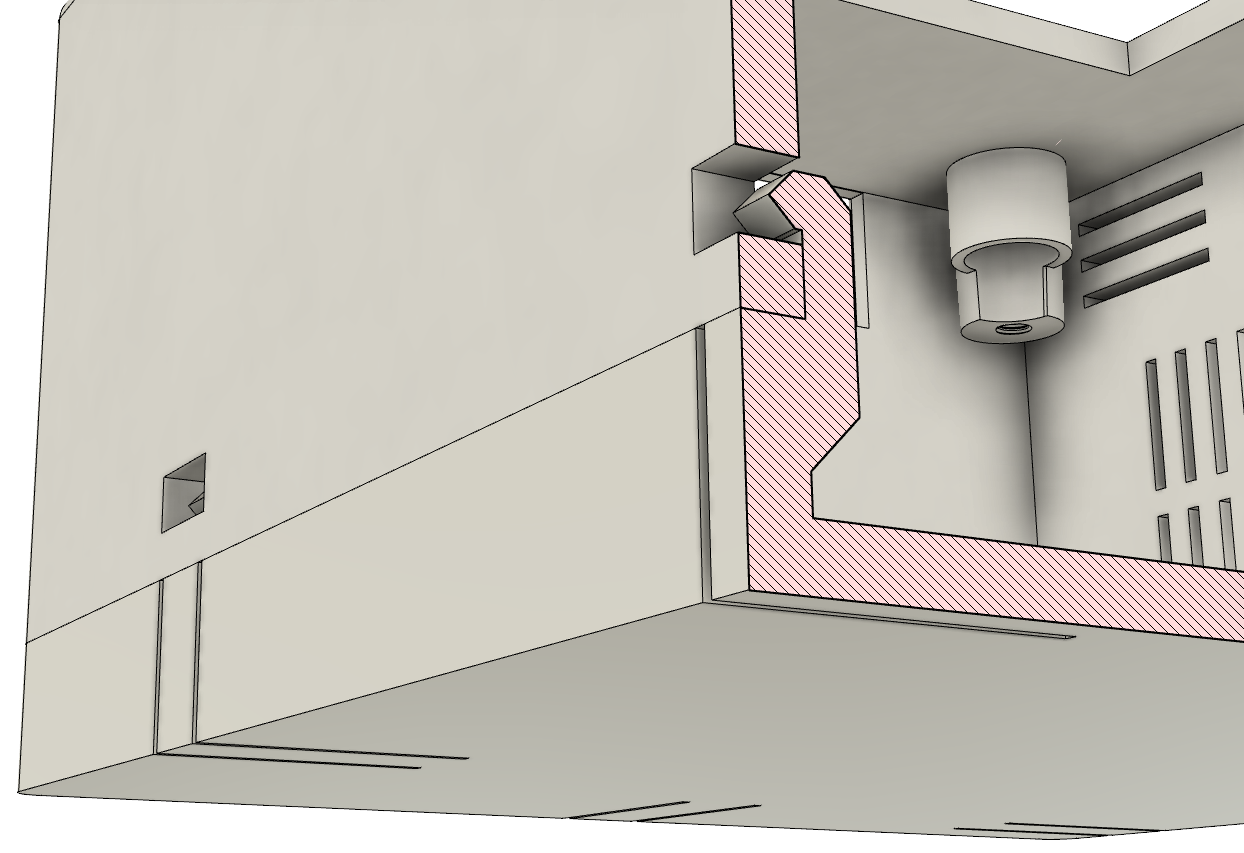
\includegraphics[height=.15\textheight]{Housing-Schnitt-Clip}
		\caption{Gehäuse Clip-Mechanismus Schnittansicht frontal}
		\label{fig:Housing-clip}
	\end{minipage}
	\hfill
	\begin{minipage}{.45\linewidth}
		\centering
		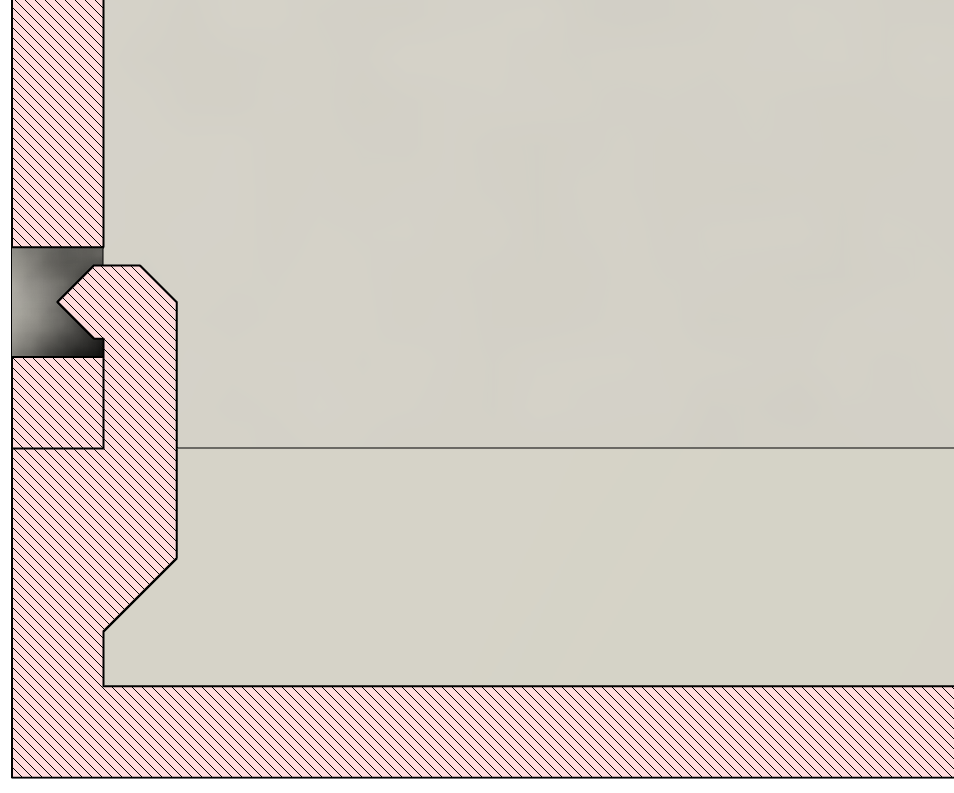
\includegraphics[height=.15\textheight]{Housing-Schnitt-Clip-Seite}
		\caption{Gehäuse Clip-Mechanismus Schnittansicht}
		\label{fig:Housing-clip-side}
	\end{minipage}
\end{figure}\\
Ein wichtiger Bestandteil der Bedienbarkeit stellen die Taster dar. Abbildung \ref{fig:Housing-btn-front} und \ref{fig:Housing-btn} zeigen den Mechanismus zum Betätigen des Tasters als Schnittansicht des 3D-Modells. Die Körper mit der Kennzeichnung 1 sind das Gehäuse an sich, die Taster sind mit 4 gekennzeichnet. Unter den Tastern befindet sich die Platine. Im Gehäuse befinden sich vier nach unten gerichtete Führungen für einen beweglichen Zylinder, welcher mit 3 gekennzeichnet ist. Alle vier Zylinder sind mit miteinander verbunden um die Stabilität zu erhöhen und ein verkanten dieser mit der Führung zu verhindern. Für die Zylinder wird ein gummiartiges Material, namens $TPU$ für den 3D-Druck verwendet, wodurch das Klicken des Tasters gedämpft wird. Die für den Benutzer sichtbaren beweglichen Taster-Flächen, gekennzeichnet mit 2, drücken den Zylinder bei einer Betätigung nach unten und diese wiederrum betätigen den Taster. Auf den Tasterflächen befinden sich Extrusionen mit der Kennzeichnung der entsprechenden Funktion des jeweiligen Tasters. Dadurch kann der Taster optisch und haptisch wahrgenommen werden, was besonders an Orten mit schlechten Beluchtungsverhältnissen wichtig ist.
%Formulierung: TPU wegen der Verbindung der Zylinder. Tasterdruck könnte mehrere Tasten betätigen
\begin{figure}[h]
	\begin{minipage}{.45\linewidth}
		\centering
		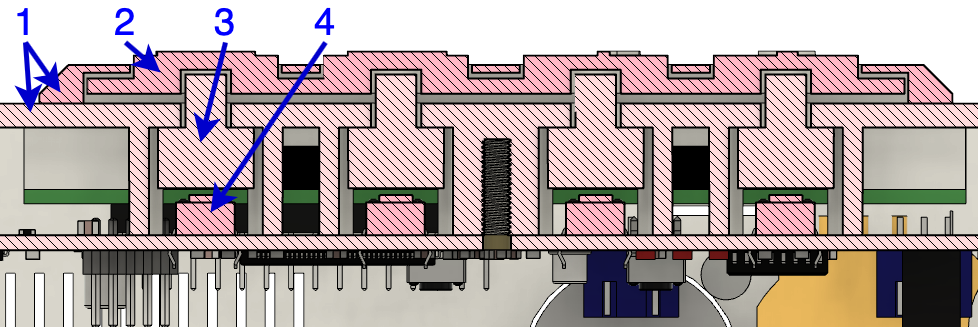
\includegraphics[width=\linewidth]{Housing-Schnitt-Button-front-crop-mark}
		\caption{Gehäuse Clip-Mechanismus}
		\label{fig:Housing-btn-front}
	\end{minipage}
	\hfill
	\begin{minipage}{.45\linewidth}
		\centering
		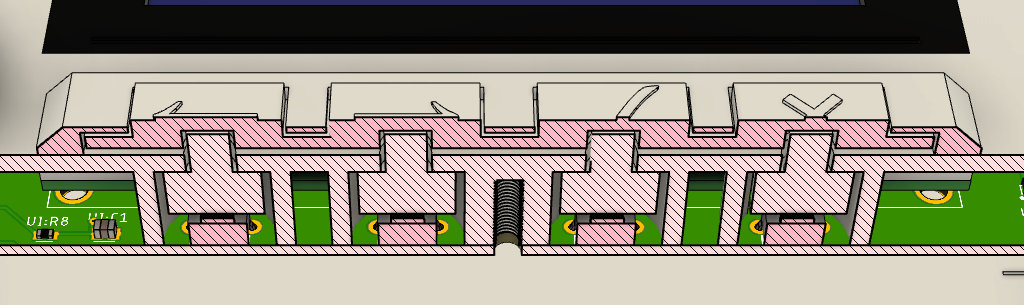
\includegraphics[width=\linewidth]{Housing-Schnitt-Button-crop}
		\caption{Gehäuse Clip-Mechanismus Schnittansicht}
		\label{fig:Housing-btn}
	\end{minipage}
\end{figure}\\